\documentclass[a4paper]{article}
\title{PHY293---Waves \& Modern Physics}
\author{Jonah Chen}


\usepackage[utf8]{inputenc}
\usepackage[margin=0.5in]{geometry}

\usepackage{braket}
\usepackage{physoly}
\usepackage{currfile}
\usepackage{gensymb}
\usepackage{amssymb}
\usepackage{pgf,tikz,pgfplots}
\usepackage{mathrsfs}
\usepackage{textcomp}
\usepackage{siunitx}
\usetikzlibrary{arrows}
\numberwithin{equation}{section}
\pgfplotsset{compat=1.16}
\everymath{\displaystyle}
\begin{document}

\maketitle
\tableofcontents
\section{Harmonic Oscillators}

\begin{itemize}
    \item Think of simple harmonic motion (SHM) as circular motion projected into one dimension. (a wave is rotation in the complex plane)
    \item One of the simplest system is a mass on the spring, with known force $F=-k\Delta x$. 
    \item For \textbf{SHM}, the motion must be periodic, and the force must be proportional to displacement.
    \item Using Newton's 2nd law on the spring force,
    \begin{align}
        m\ddot x &= -kx\\
        \ddot x + \frac{k}{m} x &= 0\label{12}
    \end{align}
    \item For a mass on the vertical spring, the equilibrium position will be lower due to gravity. 
    \begin{align}
        k(y_1-y_0)-mg&=0\\
        y_1&=y_0+\frac{mg}{k}
    \end{align}
    $y_1$ is the new equilibrium position. SHM will still occur if the system is disturbed. 
    \item Especially when dealing with energy, it is a good idea to have the origin at $y=y_1$.
\end{itemize}

\subsection{The Differential Equation}
\begin{itemize}
    \item In general, the equation for simple harmonic motion is 
    \begin{align}
        \ddot x+\omega^2 x=0
    \end{align}
    \item The solution to \eqref{12} can be represented as \begin{align}
        x=A\cos(\omega t+\varphi_0)
    \end{align} 
    \item $A$ represents the amplitude
    \item $\varphi_0$ is the phase angle (initial phase)
    \item $\omega=\sqrt{\frac{k}{m}}$ is the angular frequency.
    \item The velocity and acceleration can be easily calculated by taking derivatives.
    \begin{align}
        \dot x&=-A\omega\sin(\omega t+\varphi_0)\\
        \ddot x&=-A\omega^2\cos(\omega t+\varphi_0)
    \end{align}
    \item Another way to represent the full solution is
    \begin{align}
        x=a\cos(\omega t)+b\sin(\omega t)
    \end{align}
    where $a=A\cos\varphi_0, b=-A\sin\varphi_0$.
\end{itemize}

\begin{example}
    Determine the amplitude and phase constant of a pendulum moving with a motion described by a sum of two functions, $x_1(t)=0.25\cos\omega t$ and $x_2(t)=-0.5\sin\omega t$.
\end{example}
\begin{sol}
    \begin{align}
        0.25&=A\cos\phi_0\label{1}\\
        -0.50&=-A\sin\phi_0\label{2}
    \end{align}
    Figure out $phi_0$ from the ratio of eq.\eqref{2}/\eqref{1} % complete example
\end{sol}

\subsection{Energy of SHM}
\begin{itemize}
    \item A mass has kinetic energy of $T=\frac{1}{2}mv^2$.
    \item The potential energy is related to the restoring force and by definition,
    \begin{equation}
        \Delta U=-\int F\cdot\dd x=-\int_{x_i}^{x^f}(-kx')\dd x'=\frac{1}{2}k(x_f^2-x_i^2)
    \end{equation}
    \item The conservation of energy here follows from newton's 2nd law.
    \begin{align}
        m\ddot x=-kx % complete derivation at home
    \end{align}
    \item Looking at the potential energy
    \begin{align}
        x&=A\cos(\omega t+\varphi_0)\\
        U&=\frac{1}{2}kx^2=\frac{1}{2}kA^2\cos^2(\omega t)
    \end{align}
    \item Looking at the kinetic energy,
    \begin{align}
        T&=\frac{1}{2}mv^2=\frac{1}{2}m\omega^2A^2\sin^2(\omega t)
    \end{align}
    \item The total energy is
    \begin{align}
        E=T+\frac{1}{2}kA^2=\frac{1}{2}m\omega^2A^2=\frac{1}{2}mv_{MAX}^2
    \end{align}
\end{itemize}
\subsection{Physics of Small Vibrations}
\begin{itemize}
    \item Most system will oscillate with SHM when the amplitude is small. Recall the taylor expansion of an analytic function
    \begin{align}
        f(x)&=f(a)+(x-a)f'(a)+(x-a)^2f''(a)+\dots
    \end{align}
    If $a$ is a minima, $f'(a)=0$. For $x\approx a$, the higher order terms % complete this
    \item The potential energy of a pendulum is \begin{equation}
        U = mgy=mgL(1-\cos\theta)
    \end{equation}
    \item \textbf{For this course, an angle $\theta<\SI{10}{\degree}$, it will be considered small.}
    \item For a simple pendulum,
    \begin{align}
        -mg\sin\theta&=ma\\
        -mg\sin\theta&=m\ddot s, s=L\theta, \dd s=L\dd theta\\
        -g\sin\theta&=L\ddot\theta
    \end{align}
    For small angles, $\theta\approx\sin\theta$
    \begin{align}
        \ddot\theta+\frac{g}{L}\theta=0
    \end{align}
    This is the equation for SHM
    \item The energy of the pendulum is 
    \begin{align}
        E=T+U=\frac{1}{2}mv^2+mg\left(\frac{x^2}{2L}\right)
    \end{align}
    \item For physical pendulum, 
    \begin{align}
        \tau&=I\alpha=I\ddot\theta\\
        -mgd\sin\theta&=I\ddot\theta
    \end{align}
    For small $\theta:\sin\theta\approx\theta$
    \begin{align}
        \ddot\theta+\frac{mgd}{I}\theta=0
    \end{align}
    \item For LC circuits, 
    \begin{align}
        \ddot i+\frac{1}{LC}i=0
    \end{align}
    When a resistor is connected, energy is lost as heat and the circuit behaves like a damped oscilator.
\end{itemize}

\section{Damped Oscillations}

The damped oscillator involves the addition to the drag force that is proportional to $-v$ to the simple harmonic oscillator.

Define
\begin{align}
    \ddot x+\gamma\dot x+\omega^2x&=0\\
    x &= A\exp(\left(\sqrt{\frac{\gamma^2}{4}-\omega_0^2}-\frac{\gamma}{2}\right)t) + B\exp(-\left(\sqrt{\frac{\gamma^2}{4}-\omega_0^2}-\frac{\gamma}{2}\right)t)
\end{align}

For $\omega_0^2\neq\frac{\gamma^2}{4}$.

Critical damping gives the minimum time for the system to return to equilibrium when $\omega_0^2\neq\frac{\gamma^2}{4}$.
\begin{align}
    x=(Ax+B)\exp(-\omega_0 t)
\end{align}

\begin{example}
    A mass $m=3$ is attached to a spring with a value of $k=600$
    \begin{enumerate}
        \item Determine the value of the damping constant $b$ that would produce critical damping.
        \item Determine the value of damping constant $b$ that would decrease the angular frequency by 10\%/
        \item A mass recieve an impulse that ives it a initial velocity $v=2$. What is the maximum resultant displacement and the time when it occurs.
    \end{enumerate}
\end{example}
\begin{sol}
    \begin{enumerate}
        \item \begin{align}
            \omega_0=\frac{\gamma}{2}
        \end{align}

        \begin{align}
            x &= (A+Bt)\exp(-\frac{\gamma t}{2})\\
            \dot x&= \exp(-\frac{\gamma t}{2})\left(B-\frac{\gamma Bt}{2}-A\frac{\gamma}{2}\right)\\
        \end{align}
        $x(0)=0, \dot x(0)=v_i$
        \begin{align}
            x &=v_i t\exp(-\frac{\gamma t}{2})\\
            \dot x &= v_i\exp(-\frac{\gamma t}{2})\left(1-\frac{\gamma t}{2}\right) = 0\\
            t &= \frac{2}{\gamma}=\frac{2m}{b}\\
            x\left(\frac{2}{\gamma}\right)&=v_it\exp(-\frac{\gamma t}{2})=\frac{2v_i}{\gamma e}
        \end{align}
    \end{enumerate}
\end{sol}

\subsection{Energy}
For underdamped oscillator, assume $\omega\approx\omega_0$.
\begin{align}
    E&=T+U=\frac{1}{2}mv^2+\frac{1}{2}kx^2\\
    x&=A_0\exp((i\omega_0-\frac{\gamma}{2})t)\\
    \dot x&=-A_0\exp(t\left(i\omega_0-\frac{\gamma}{2}\right))=A_0\left(i\omega_0-\frac{\gamma}{2}\right)\exp(t\left(i\omega_0-\frac{\gamma}{2}\right))\\
    E&=\frac{1}{2}kA_0^2\exp(-\gamma t)\\
\end{align}

The rate of change of energy is 
\begin{align}
    \dot E=\frac{\dd}{\dd t}\left(\frac{1}{2}mv^2+\frac{1}{2}kx^2\right)=\dot x(m\ddot x+k\dot x)
\end{align}
Recall $m\ddot x=-kx-b\dot x$
\begin{align}
    \dot E=-b\dot x^2=-\gamma E 
\end{align}

\begin{example}
    The energy of a simple harmonic oscillator is ovserved to reduce by a factor of two after 10 complete cycles.
    \begin{enumerate}
        \item How amny cycles will it take to reduce it by a factor of 8?
        \item By what factor would it be reduced after 100 cycles?
    \end{enumerate}
\end{example}
\begin{sol}
    \begin{enumerate}
        \item \begin{align}
            \frac{E}{E_0}&=e^{-\gamma t}\\
            \frac{1}{2}&=e^{-\gamma 10 T}\\
            \left(\frac{1}{2}\right)^3&=\left(e^{-\gamma 10 T}\right)^3=e^{-\gamma 30 T}
        \end{align}
    \end{enumerate}
\end{sol}

\subsection{Quality Factor}

\begin{definition}
    The \textbf{quality factor} is a convenient measurement on how good an oscillator is (how many oscillations it can make before its amplitude would decrease by a certain rate) is defined as 
    \begin{equation}
        Q=\frac{\omega_0}{\gamma}=\frac{\sqrt{km}}{b}
    \end{equation}
    where $\gamma=2\beta=\frac{b}{m}$.
\end{definition}
\begin{itemize}
    \item If $Q=\frac{1}{2}$, the system is critically damped.
    \item Energy $E=E_0\exp(-\gamma t)$.
    \item At two different times $t_1$ and $t_2$ seperated by period $T$, 
    \begin{align}
        \frac{E(t+T)}{E(t)}=\exp(-\gamma T)
    \end{align}
    Which leads to
    \begin{align}
        \frac{E(t)-E(t+T)}{E(t_1)}=1-e^{-\gamma T}\approx -\gamma T\approx\frac{2\pi\gamma}{\omega}=\frac{2\pi}{Q}
    \end{align}
    Thus,
    \begin{align}
        Q=\frac{\text{Energy stored in the oscillator}}{\text{Energy dissipated per radian}}
    \end{align}
    \item We can rewrite the equation of the damped oscillator
    \begin{align}
        \ddot x+\gamma\dot x+\omega_0^2 x&=0\\
        \ddot x+\frac{\omega_0}{Q}\dot x+\omega_0^2 x&=0
    \end{align}
    As $\displaystyle{\gamma=\frac{\omega_0}{Q}, \omega=\omega_0\sqrt{1-\frac{1}{4Q^2}}}$.
    \begin{center}
        \begin{tikzpicture}
            \begin{axis}[xlabel=$Q$,ylabel=$\omega/\omega_0$]
                \addplot [
                    domain=0:10,
                    samples=200,
                    color=blue,
                    ]
                    {sqrt(1-0.25*x^(-2))};
            \end{axis}
        \end{tikzpicture}
    \end{center}
\end{itemize}
\begin{example}
    WHen an electron in $H$ is moved from $n=2$ to $n=3$ states, the atom behaves like a damped oscillator when the lights of frequency \SI{4.57e+14}{\hertz} is emmited. The lifetime of the excited atom is approximately \SI{10}{\nano\second}. What is the value of the quality factor?
\end{example}
\begin{sol}
    As $\gamma=\frac{1}{\tau}, \omega_0=2\pi f$, 
    \begin{equation}
        Q=\frac{\omega_0}{\gamma}=2\pi f\tau=\SI{2.87e+7}{}
    \end{equation}
\end{sol}
\begin{itemize}
    \item RLC circuit:
    \begin{align}
        RI+L\dot I+\frac{q}{C}&=0\\
        L\ddot q+R\dot q+\frac{q}{C}&=0\\
        \ddot q+\frac{R}{L}\dot q+\frac{1}{LC}q&=0
    \end{align}
\end{itemize}
\section{Driven Oscillations}
In the undamped case,
\begin{align}
    m\ddot x+kx&=F_0e^{i\omega t}\\
    m\ddot x+kx&=ka e^{i\omega t}\\
\end{align}
The particular solution is 
\begin{align}
    x=A(\omega)e^{i(\omega t-\delta)}
\end{align} 
where
\begin{itemize}
    \item $\tan\delta=0$ and $A(\omega)=\frac{a}{1-(\omega/\omega_0)^2}$ when $\omega<\omega_0$
    \item $\tan\delta=\pi$ and $A(\omega)=-\frac{a}{1-(\omega/\omega_0)^2}$ when $\omega>\omega_0$
\end{itemize}

\subsection{With damping}

\begin{align}
    \ddot x+\gamma\dot x+\omega_0^2&=ae^{i\omega t}
\end{align}
Solving for $x$, the particular solution is
\begin{align}
    x=A(\omega)e^{i(\omega t-\delta)}
\end{align}
with $\tan\delta=\frac{\omega\gamma}{\omega_0^2+\omega^2}$, $A(\omega)=\frac{a\omega_0^2}{\sqrt{(\omega_0^2-\omega^2)^2+(\omega\gamma)^2}}$. %This is DAF for civ102
\begin{center}
    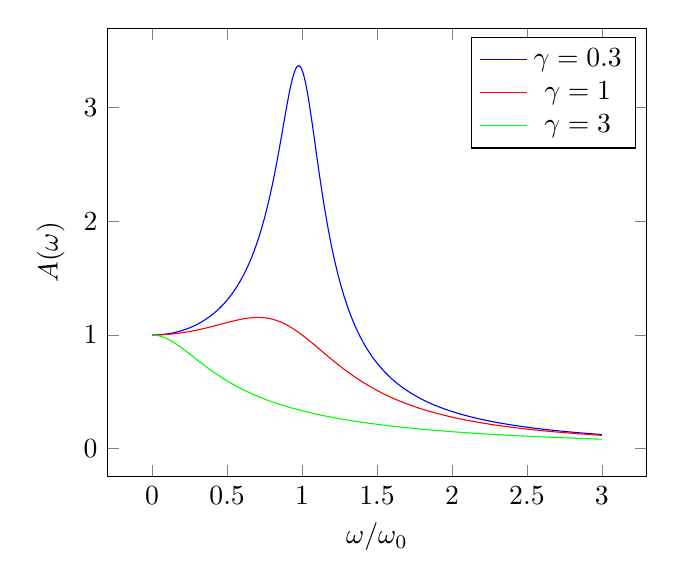
\begin{tikzpicture}% coordinates%\begin{}[]%\addplot coordinates {};%\end{}%\end{}
        \begin{axis}[xlabel=$\omega/\omega_0$,ylabel=$A(\omega)$]
            \addplot [
                domain=0:3,
                samples=200,
                color=blue,
                ]
                {1/sqrt((1-x^2)^2+0.3*0.3*x*x)};
            \addlegendentry{$\gamma=0.3$}
            \addplot [
                domain=0:3,
                samples=200,
                color=red,
                ]
                {1/sqrt((1-x^2)^2+x*x)};
            \addlegendentry{$\gamma=1$}
            \addplot [
                domain=0:3,
                samples=200,
                color=green,
                ]
                {1/sqrt((1-x^2)^2+9*x*x)};
            \addlegendentry{$\gamma=3$}
        \end{axis}
    \end{tikzpicture}
    \begin{tikzpicture}% coordinates%\begin{}[]%\addplot coordinates {};%\end{}%\end{}
        \begin{axis}[]
            \addplot [
                domain=0:3,
                samples=200,
                color=blue,
                ]
                {atan(1/sqrt(abs(x^2-1)))};            
        \end{axis}
    \end{tikzpicture}
\end{center}

If it is driven at the resonance frequency, 
\begin{align}
    A&=\frac{a\omega_0}{\gamma}\\
    \delta&=\frac{\pi}{2}
\end{align}

For large damping, $\omega_{max}\neq\omega_0$.

\subsection{Power}

If the motion of a driven oscillator is
\begin{equation}
    x=A(\omega)e^{i(\omega t-\delta)}
\end{equation}
The velocity is 
\begin{equation}
    \dot x=iA(\omega)\omega e^{i(\omega t-\delta)}
\end{equation}
Note that power lost to damping is 
\begin{equation}
    P=b\dot x^2
\end{equation}
The full width at half height of the period-averaged power is $\gamma/\omega_0=\frac{1}{Q}$
\begin{center}
    \begin{tikzpicture}% coordinates%\begin{}[]%\addplot coordinates {};%\end{}%\end{}
        \begin{axis}
            \addplot [
                domain=0:2,
                samples=70,
                color=blue,
                ]
                {x^2/((x-1)^2+0.3*x*x)};            
        \end{axis}
    \end{tikzpicture}
\end{center}

If the driving frequency is close to the natural frequency, 
\begin{equation}
    (\omega^2-\omega_0^2)=(\omega-\omega_0)(\omega+\omega_0)\approx -2\omega_0\Delta\omega
\end{equation}
Then, 
\begin{equation}
    \overline P(\omega)=\frac{F_0^2}{2m\gamma[\frac{4\Delta\omega^2}{\gamma^2}+1]}
\end{equation}
\subsection{Reasonance in RLC circuits}
\begin{align}
    RI+L\dot I+\frac{q}{C}&=\varepsilon_0\cos(\omega t)\\
    L\ddot q+R\dot q+\frac{q}{C}&=\varepsilon_0\cos(\omega t)\\
    \ddot q+\frac{R}{L}\dot q+\frac{1}{LC}q&=\frac{\varepsilon_0}{L}\cos(\omega t)
\end{align}
$$\omega_0^2=\frac{1}{LC},\gamma=\frac{R}{L},Q=\frac{\omega_0}{\gamma}=\sqrt{\frac{L^2}{RC}}$$
\begin{align}
    q(t)&=q_0(\omega)e^{i(\omega t-\delta)}\\
    q_0(\omega)&=\frac{\varepsilon_0}{L\sqrt{(\omega_0^2-\omega^2)^2+\left(\frac{R\omega}{L}\right)^2}}=\frac{\varepsilon_0}{\omega\sqrt{\left(\frac{1}{\omega C}-\omega L\right)^2+R^2}}
\end{align}

\subsection{Transient Phenomena}

When the driving force is first applied and the system is distributed from equilibium the system will be inclined to oscillate at its natural frequency, especially if the system is delicate.This is shown by the homogenous solution of the differential equation. 

\section{Coupled Oscillator}
\begin{itemize}
    \item For a system of coupled oscillators can be described by equations
    \begin{align}
        m_1\ddot x_1 &= k_{11}x_1 + \dots + k_{1n}x_n\\
        &\vdots\\
        m_n\ddot x_n &= k_{n1}x_1 + \dots + k_{nn}x_n
    \end{align}
    Thus, \begin{align}
        M\ddot x=Kx
    \end{align}
\end{itemize}
\end{document}
